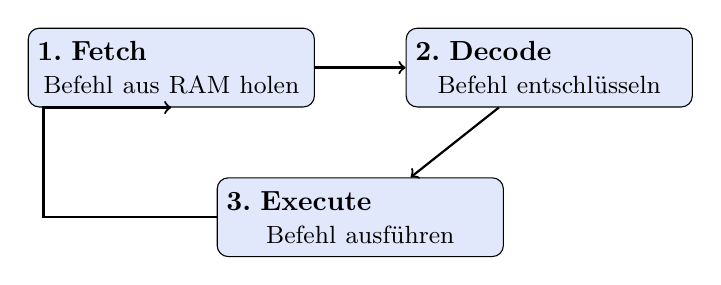
\begin{tikzpicture}[
    block/.style={draw, rounded corners, minimum width=3.4cm, minimum height=1.0cm, text centered, text width=3.4cm, fill=RoyalBlue!15},
    arrow/.style={->, thick}
]
    \node[block] (fetch)   at (0, 0)    {\textbf{1.\ Fetch} \newline \small Befehl aus RAM holen};
    \node[block] (decode)  at (4.8, 0)  {\textbf{2.\ Decode} \newline \small Befehl entschlüsseln};
    \node[block] (execute) at (2.4,-1.9) {\textbf{3.\ Execute} \newline \small Befehl ausführen};

    \draw[arrow] (fetch)   -- (decode);
    \draw[arrow] (decode)  -- (execute);
    \draw[arrow] (execute.west) -- ++(-2.2,0) |- (fetch.south);
\end{tikzpicture}
